\subsection{Resolver}\label{subsubsec:Resolver}

Damit die genaue Lage des Rotors festgestellt werden kann, benötigt es eine Drehpositionserfassung. Im Falle des verwendeten Motors wird ein Koordinatenwandler, auf Englisch auch Resolver genannt, verwendet.
Dieser hat die Eigenschaft, eine kontinuierliche Winkellage des Rotors zu liefern und ist fest im AKM22h verbaut. Aus diesem Grund wird in diesem Kapitel die Funktion des Resolvers vertieft betrachtet.

\subsubsection{Aufbau}\label{par:Aufbau_Resolver}

Damit ein Resolver funtionieren kann, sind eine Erregerspule und zwei Sensorspulen nötig.
Weiter muss mittels Induktion die Erregungsfrequenz auf die Erregerspule übertragen werden.
Der schematische Aufbau ist in Abbildung  \ref{fig:Schematisch_Grafisch_Resolver_1} ersichtlich. Abbildung \ref{fig:Schematisch_Grafisch_Resolver_2} zeigt, wie die Komponenten zu einander stehen und wie sie (bis auf die blaue Leiterschleife) im Resolver angeordnet sind.

Das Prinzip funktioniert folgendermassen. Es wird ein periodisches Signal, vorzugsweise Sinus, auf die statische gelbe Spule gegeben. Dieses wird mittels Induktion des drehbaren Transformators an die drehbare blaue Spule übertragen. Die blaue Spule erzeugt unabhängig ihrer Lage ein magnetisches Feld anhand des Erzeugersignals und bildet so die Erregerspule. Die grüne und pinke Sensorspulen werden je nach Lage der blauen Spule unterschiedlich stark erregt und erzeugen das benötigte Signal, welches dann von der Auswertelektronik verarbeitet wird. 

\begin{figure}[h!]
\centering
\subcaptionbox{Schematische Darstellung Resolver\cite{noauthor_wie_nodate}\label{fig:Schematisch_Grafisch_Resolver_1}}{	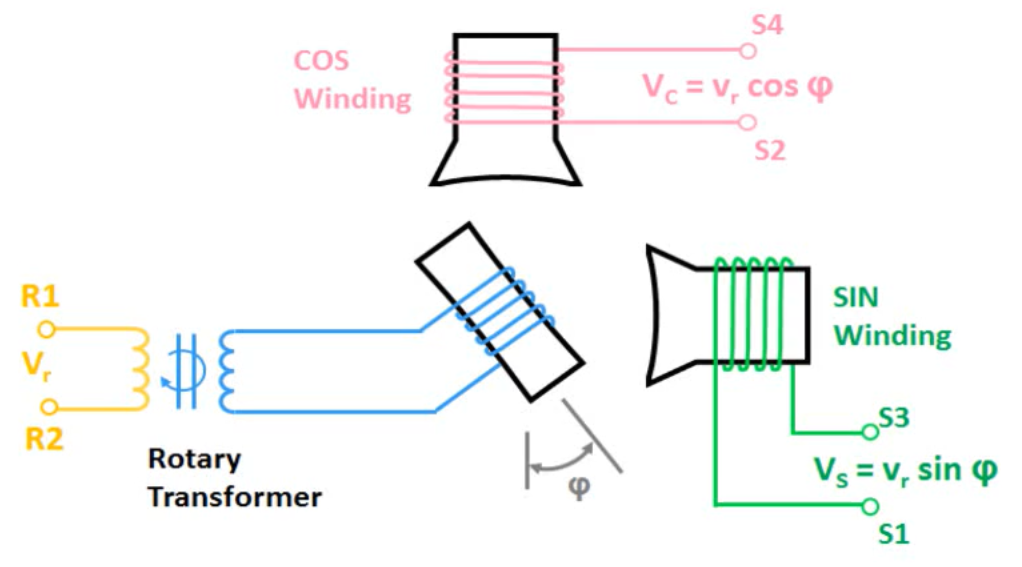
\includegraphics[width=0.45\textwidth]{graphics/Resolver_1.png}}
\hfill
\subcaptionbox{Grafische Darstellung Resolver\cite{noauthor_wie_nodate}\label{fig:Schematisch_Grafisch_Resolver_2}}{	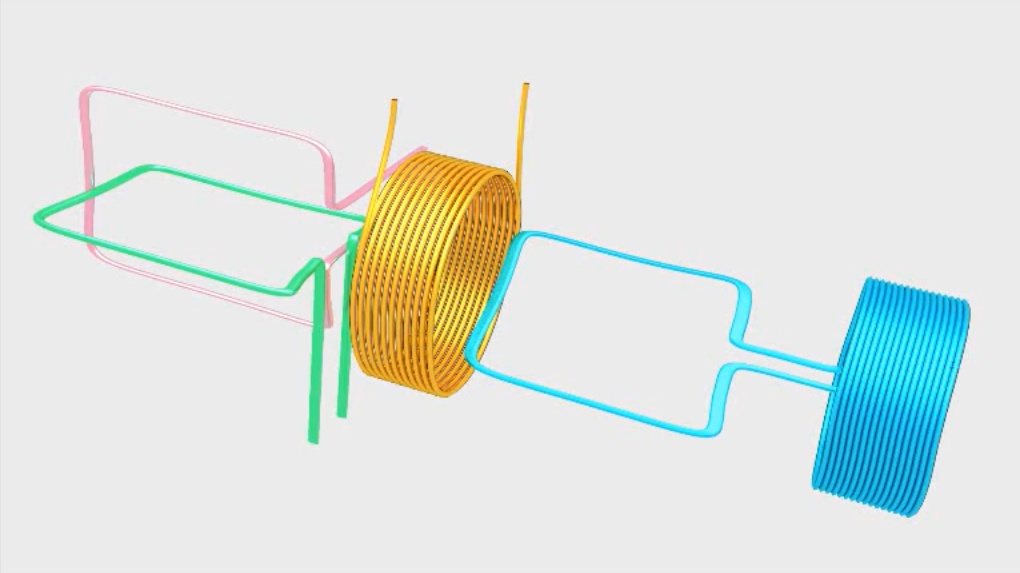
\includegraphics[width=0.45\textwidth]{graphics/Resolver_2.png}}
\hfill
\caption{Schematische und grafische Darstellung eines Resolvers.}
\label{fig:Schematisch_Grafisch_Resolver}
\end{figure}

\subsubsection{Funktionsweise}\label{par:Funktionsweise_Resolver}

Steht der Rotor wie in Abbildung \ref{fig:Position_Grafisch_0} bei 0$^\circ$, so liegt die drehbare blaue Leiterschleife so, dass der von ihr ausgehende magnetische Fluss nur eine Wirkung auf die pinke Leiterschleife hat (siehe Abbildung \ref{fig:Darstellung_Grafisch_0}). Das Erregersignal wird folglich praktisch nur von der cos-Windung wahrgenommen, wie in Abbildung \ref{fig:Signal_Grafisch_0} ersichtlich ist.

\begin{figure}[h!]
\centering
\subcaptionbox{Grafische Lage der Spulen\cite{noauthor_wie_nodate}\label{fig:Darstellung_Grafisch_0}}{	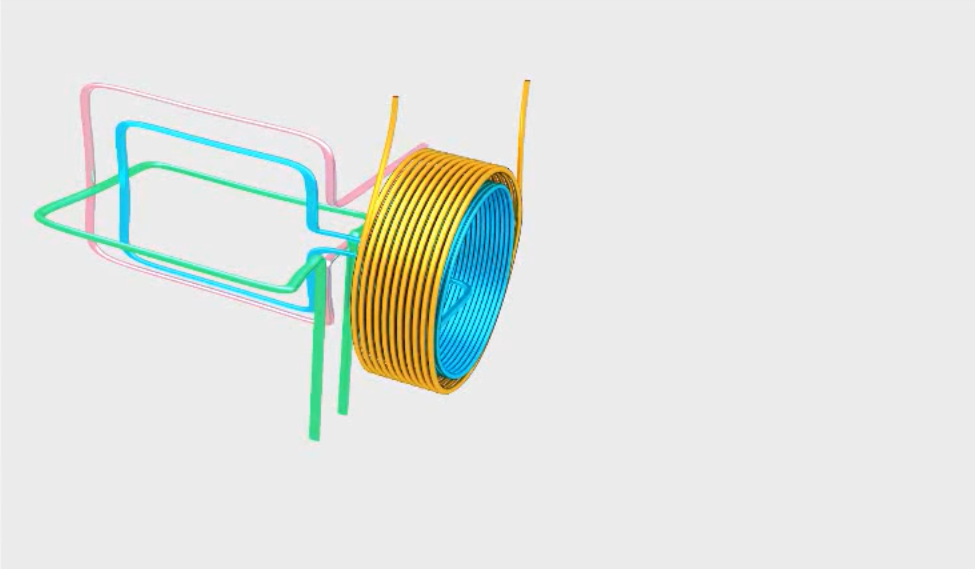
\includegraphics[width=0.3\textwidth]{graphics/Resolver_3.png}}
\hfill
\subcaptionbox{Signalverläufe der Spulen\cite{noauthor_wie_nodate}\label{fig:Signal_Grafisch_0}}{	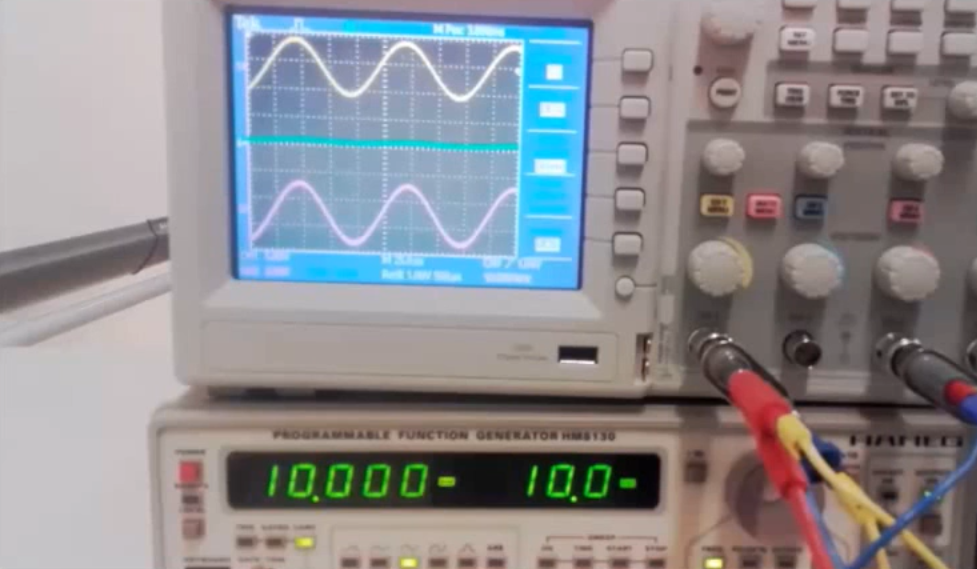
\includegraphics[width=0.3\textwidth]{graphics/Resolver_5.png}}
\hfill
\subcaptionbox{Position des Resolvers\cite{noauthor_wie_nodate}\label{fig:Position_Grafisch_0}}{	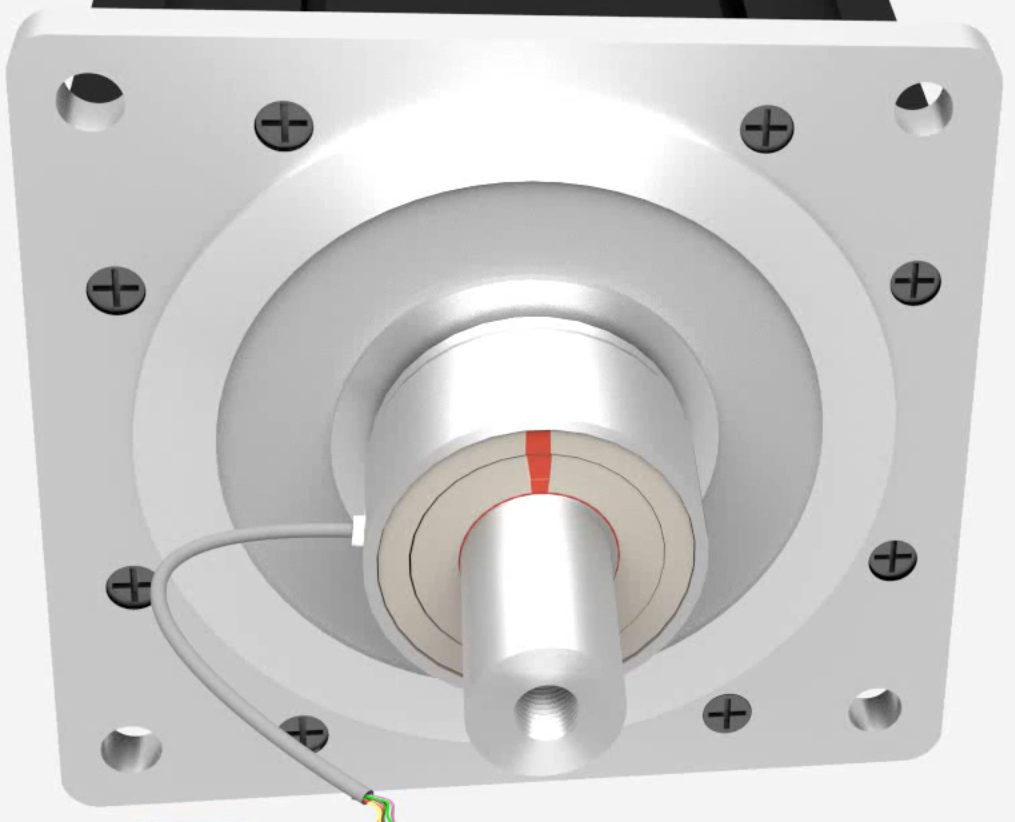
\includegraphics[width=0.3\textwidth]{graphics/Resolver_7.png}}
\hfill
\caption{Gegebenheiten bei Achsenstellung 0$^\circ$.}
\label{fig:Darstellungen_0_Grad}
\end{figure}

Steht der Rotor wie in Abbildung \ref{fig:Position_Grafisch_90} bei 90$^\circ$, so liegt die drehbarebare blaue Leiterschleife so, dass der von ihr ausgehende magnetische Fluss nur eine Wirkung auf die grüne Leiterschleife hat (siehe Abbildung \ref{fig:Darstellung_Grafisch_90}). Das Erregersignal wird folglich praktisch nur von der sin-Windung wahrgenommen, wie in Abbildung \ref{fig:Signal_Grafisch_90} ersichtlich.

\begin{figure}[h!]
\centering
\subcaptionbox{Grafische Lage der Spulen\cite{noauthor_wie_nodate}\label{fig:Darstellung_Grafisch_90}}{	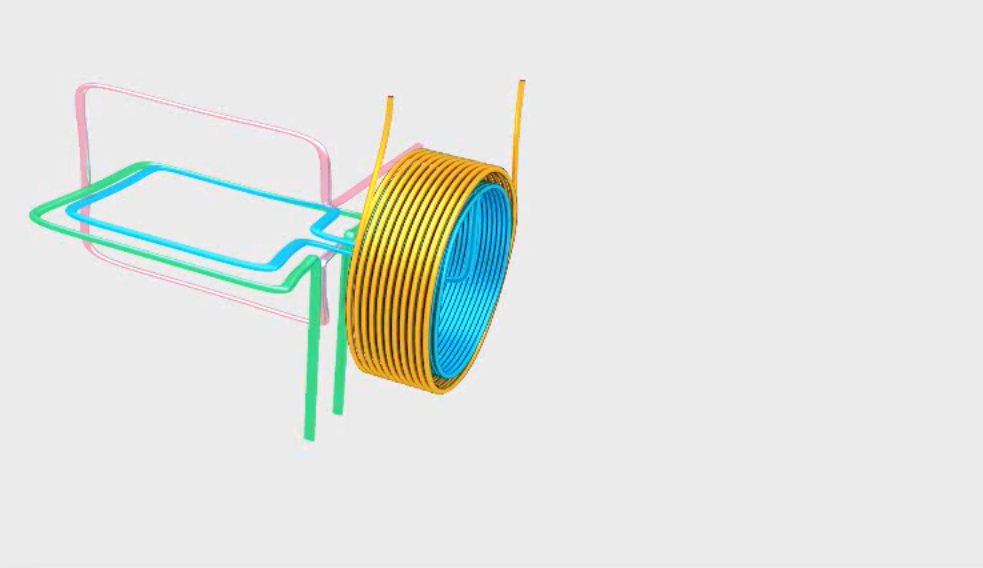
\includegraphics[width=0.3\textwidth]{graphics/Resolver_4.png}}
\hfill
\subcaptionbox{Signalverläufe der Spulen\cite{noauthor_wie_nodate}\label{fig:Signal_Grafisch_90}}{	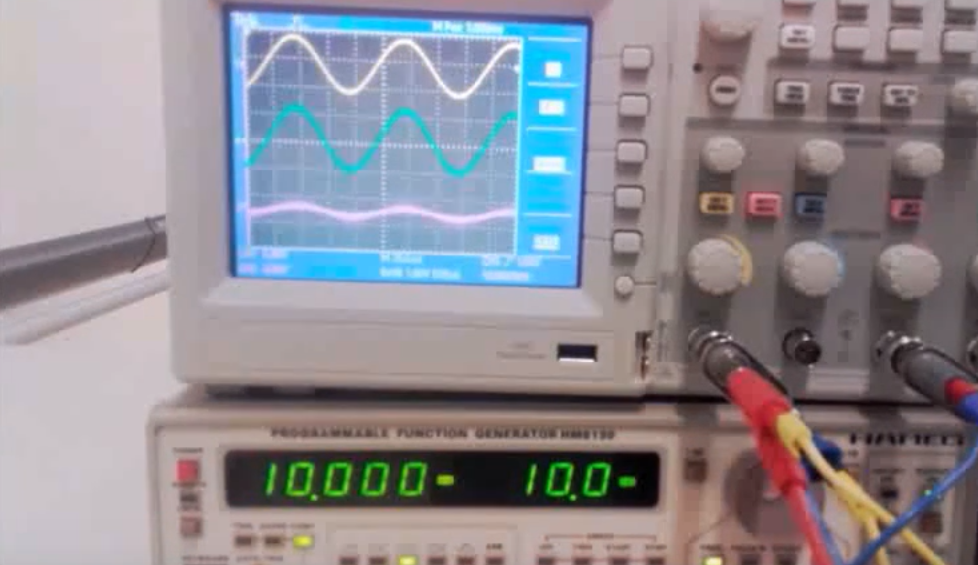
\includegraphics[width=0.3\textwidth]{graphics/Resolver_6.png}}
\hfill
\subcaptionbox{Position des Resolvers\cite{noauthor_wie_nodate}\label{fig:Position_Grafisch_90}}{	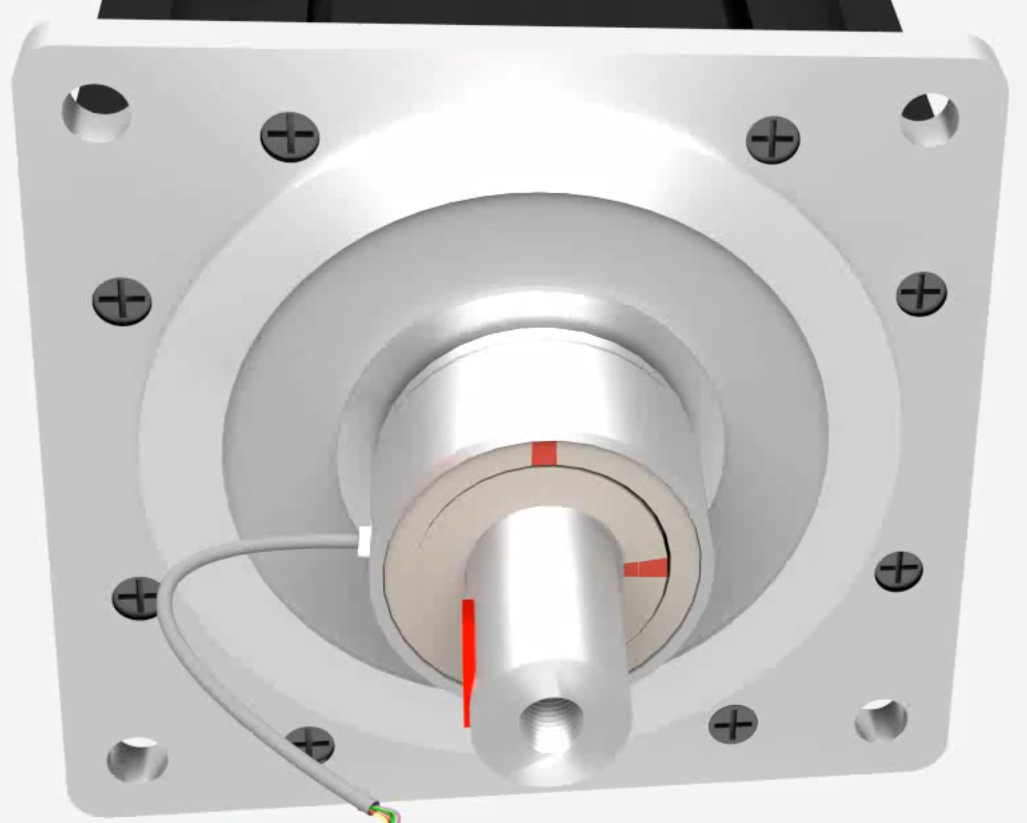
\includegraphics[width=0.3\textwidth]{graphics/Resolver_8.png}}
\hfill
\caption{Gegebenheiten bei Achsenstellung 90$^\circ$.}
\label{fig:Darstellungen_90_Grad}
\end{figure}